\section{Proof of Concept}

Zum Testen eines approximativen Algorithmus wurde sich für das Zählen unterschiedlicher Elemente mithilfe des HyperLogLog-Algorithmus entschieden.
Als Datenquelle werden die Änderungen von Wikipedia-Artikeln beobachtet, um so zu approximieren, wie viele unterschiedliche Artikel täglich geändert werden.
Die Streambeobachtung des Proof of Concept ist im Anhang in \autoref{lst:wikistream} dargestellt.

Die Wikimedia Foundation bietet EventStreams für diverse Änderungen an.
Für dieses Beispiel wichtig ist der unter \url{https://stream.wikimedia.org/v2/stream/recentchange} gelieferte Stream über alle Seitenänderungen.
Da der Stream Änderungen an diversen Wikis der Wikimedia Foundation überträgt, werden die einkommenden Events nach der Domain ,,wikipedia.org`` gefiltert.

Die Seitennamen der eingehenden Events werden dann auf drei verschiedene Arten gespeichert:  in einer Menge, um so eine naive Implementierung und einen Vergleichswert mit den Alternativen herzustellen, in einer bestehenden Implementierung des HyperLogLog-Algorithmus aus der gleichnamigen Python-Bibliothek \cite{evseenko2018} und in einer minimalen, eigenen Implementierung des Algorithmus, zu sehen im Anhang in \autoref{lst:hyperloglog}.
Die Genauigkeit des HyperLogLog-Algorithmus kann dabei proportional zum Speicherplatzbedarf gesteigert werden.
Dies erlaubt eine variable Genauigkeit.
Bei beiden verwendeten Algorithmen wurde deshalb eine maximale Abweichung von 1\% erlaubt.

Der Stream wurde über einen Zeitraum von 24~Stunden beobachtet und die Daten mitgeschrieben.
Anschließend wurden Informationen zum Speicherverbrauch und der Genauigkeit der beiden HyperLogLog-Implementierungen analysiert.

\subsection{Funktionsweise und Implementierung}
\label{sec:proof-of-concept-funktionsweise}

\begin{figure*}[b]
	\centering
	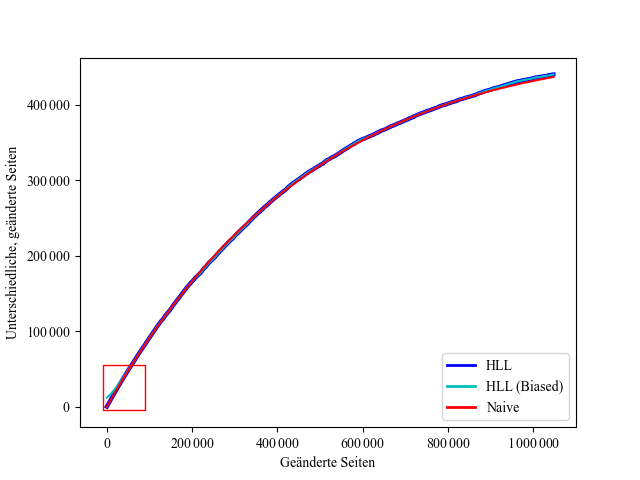
\includegraphics[width=.49\textwidth]{images/hll_count_1.png}
	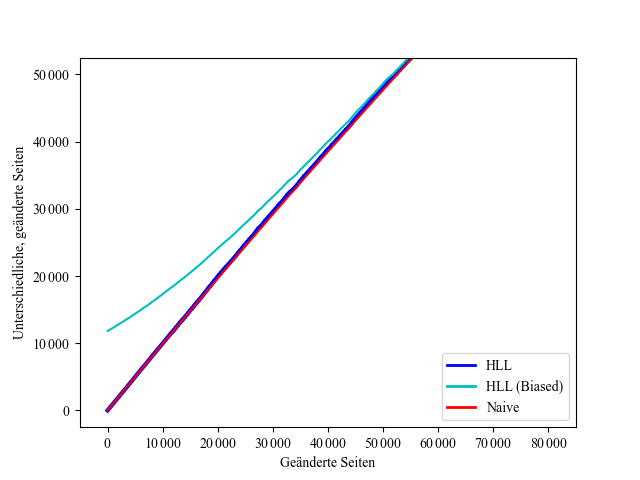
\includegraphics[width=.49\textwidth]{images/hll_count_2.png}
	\caption{Genauigkeit naiver Implementierung gegenüber HyperLogLog}
	\label{fig:hll-count}
\end{figure*}

Beim HyperLogLog-Algorithmus werden eingehende Daten mit einer Hash-Funktion in eine zufällige Reihe aus Bits $\{0, 1\}^\infty$ umgewandelt.
Abhängig von der gewünschten Genauigkeit wird dann eine bestimmte Anzahl $b$ Bits weggenommen.
Diese Bits ergeben die binäre Speicheradresse eines Registers.
Dies führt zu $m=2^b$ unterschiedlichen Registern.
Je höher diese Zahl ist, desto genauer wird die Schätzung des Algorithmus.
Von den übrig bleibenden Bits des Hashes wird die Position von links des höchstwertigen 1-Bit bestimmt und in das entsprechende Register geschrieben.
Sollte das Register bereits einen höheren Wert enthalten, wird der alte Wert beibehalten.
Aus diesen Registern wird bei Abfrage ein stochastischer Erwartungswert berechnet, welcher der Anzahl unterschiedlicher, eingefügter Elemente entsprechen soll \cite{flajolet2007}.

Für den Algorithmus berechnet sich eine Abweichung abhängig von der Anzahl der Register $e=1.04/\sqrt{m}$ \cite{flajolet2007}.
Somit kann im Umkehrschluss auch die benötigte Anzahl an Registern und führenden Bits -- und somit auch der Speicherplatzbedarf -- aus einer gegebenen maximalen Abweichung wie in Gleichung~\eqref{eq:target-error} dargestellt berechnet werden.
Im Beispiel dieses Proof of Concept benötigt die gewählte Genauigkeit von einem Prozent $b = log_2 (\frac{1.04}{0.01})^2 = 13.40$, beziehungsweise aufgerundet 14 führende Bits des Hashes.
Dies führt zu $m = 2^{14} = 16\,384$ benötigten Registern und somit einem maximalen Speicherverbrauch von 16\,384~Byte.

\begin{equation}
	\begin{alignedat}{2}
		& e & \: = \: & \frac{1.04}{\sqrt{m}} \\
		\Rightarrow \: & m & \: = \: & \left(\frac{1.04}{e}\right)^2 = 2^b \\
		\Rightarrow \: & b & \: = \: & \log_2 m = \log_2 \left(\frac{1.04}{e}\right)^2
	\end{alignedat}
	\label{eq:target-error}
\end{equation}

\subsection{Ergebnis der Streambeobachtung}

Bei der Beobachtung ergab sich im Bereich bis etwa 50\,000 einzigartiger Einträge eine starke Abweichung des selbst implementierten HyperLogLog-Algorithmus (siehe \autoref{fig:hll-count}).
So erreichte dieser die gewünschte Genauigkeit von 99\% erst bei 44\,162 einzigartigen Einträgen.
Ab diesem Eintrag verhielten sich beide Implementierungen, die eigene und die von Evseenko \cite{evseenko2018}, sehr ähnlich, jedoch erst ab dem 398\,115. einzigartigen Eintrag vollkommen identisch.

Diese Abweichung entstammt einem Bias des HyperLogLog-Algorithmus, weshalb niedrige Kardinalitäten stark überschätzt werden \cite{heule2013}.
Um diesem Problem entgegenzuwirken, kann eine Linear-Counting-Funktion unterhalb einer gewissen Schwelle eingesetzt werden, was auch in der bezogenen Implementierung verwendet wird \cite{evseenko2018}.

Der gemessene Speicherbedarf bei der HyperLogLog-Implementierung lag, wie in \autoref{fig:hll-memory} dargestellt, stabil bei den zuvor berechneten 16\,384~Byte.
Demhingegen steigt der Speicherverbrauch der naiven Python-Implementierung in einer Menge rasant an.
Zu beachten ist hierbei die logarithmische Skala der Abbildung.
So steigt der Speicherbedarf des Python-Sets schon beim Einfügen des 309.
Elements auf das Doppelte des HyperLogLog-Speicherbedarfs und bis zum Ende auf das Zehnfache.

\begin{figure}[t]
	\centering
	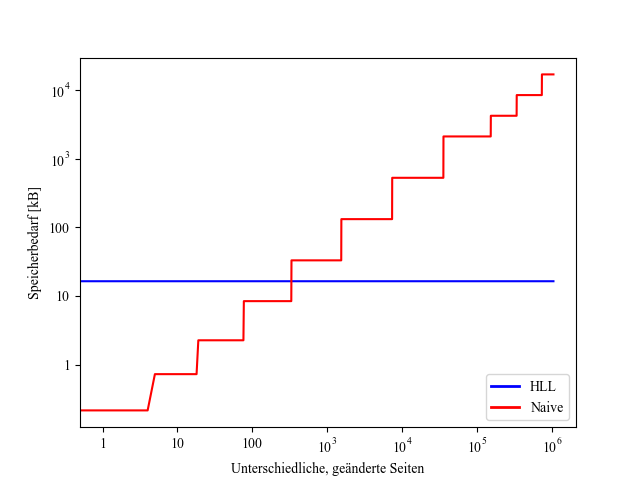
\includegraphics[width=0.49\textwidth]{images/hll_memory.png}
	\caption{Speicherbedarf naiver Implementierung gegenüber HyperLogLog}
	\label{fig:hll-memory}
\end{figure}

Der Vorteil des HyperLogLog-Algorithmus stellt sich klar im Bereich größerer Datenmengen heraus.
Durch den konstanten Speicherverbrauch und eine hohen Präzision bei größeren Datenmengen bietet sich der Algorithmus hier an, da bei naiver Datenspeicherung in einer Menge der benötigte Speicher stark ansteigt.
Flajolet et al. \cite{flajolet2007} beschreiben eine gute Approximation für Kardinalitäten $N \le 10^9$.
Ein Test mit Kardinalität dieser Größenordnung konnte aus technischen Gründen nicht durchgeführt werden.

Da der Hauptteil der Approximation erst bei der Abfrage durchgeführt wird, ist das Hinzufügen eines Wertes zu einem HyperLogLog-Speicher außerdem sehr schnell.
Im durchgeführten Test ergab sich für die naive Implementierung mit einer Menge eine durchschnittliche Zeit der Größenordnung 10\textsuperscript{-7}\,Sekunden (100\,ns), für die HyperLogLog-Varianten je 10\textsuperscript{-6}\,Sekunden (1\,\textmu{}s).
Das Abfragen der Länge ging jedoch erwartungsgemäß etwas länger.
Die Länge der Menge wurde in einer Größenordnung von 10\textsuperscript{-8}\,Sekunden (10\,ns) ermittelt, wobei die Approximationen je im Bereich 10\textsuperscript{-3} bis 10\textsuperscript{-2}\,Sekunden (1--10\,ms) lagen.